% !TeX spellcheck = ru_RU

\section{Эксперимент}

После реализации алгоритма было необходимо протестировать его работоспособность на данных из реального мира и сравнить его производительность с реализацией на CPU, чтобы понять, что дал перенос алгоритма для вычислений на видеокарте.

В качестве данных была выбрана база знаний \textsc{Wikidata}\footnote{База знаний \textsc{WikiData}: \href{https://www.wikidata.org/wiki/Wikidata:Database_download}{https://www.wikidata.org/wiki/Wikidata:Database\_download} (Дата доступа 11.12.24)} \cite{wikidata}, на которой тестировалась производительность реализации на CPU в работе ~\cite{OldRpqVkr}, так как это один из самых разнообразных и больших графов доступных публично и вместе с ним доступны наборы реальных регулярных запросов. Код\footnote{Код для теста производительности алгоритма: \url{https://github.com/georgiy-belyanin/RPQ-bench} (Дата посещения: 08.01.2025)} для теста производительности выложен автором алгоритма на GitHub.

\subsection{Условия эксперимента}
Эксперименты проводились на тестовом стенде со следующей конфигурацией.
\begin{itemize}
    \item \textbf{CPU}: Intel i5-10400f, 6 физических, 12 логических ядер, максимальная частота 4.3 GHz
    \item \textbf{GPU}: Nvidia RTX 3050, 8 Gb VRAM, 1552 MHz
    \item \textbf{RAM}: 16 Gb, 3200 MHz, DDR4
    \item \textbf{OS}: Ubuntu 24.04
    \item \textbf{Компиляторы}: nvcc 12.6, gcc 14.2
\end{itemize}
Измерялось только время работы алгоритма, загрузка входных данных в оперативную память и видеопамять не учитывалась.

Тестирование проводилось на 520 запросах, среди которых встречаются двусторонние. Размеры графа порядка $10^8$, что позволяет протестировать алгоритм на графe большого размера.

Погрешности измерения не указаны, так как они достаточно малы.
Для каждого алгоритма все запросы были проведены по 10 раз, и стандартное отклонение только у 1 запроса для GPU превысило 1\%, для измерений на CPU у 6 запросов, но ни одно стандартное отклонение не превысило 8\%.

\begin{figure}[H]
    \centering
    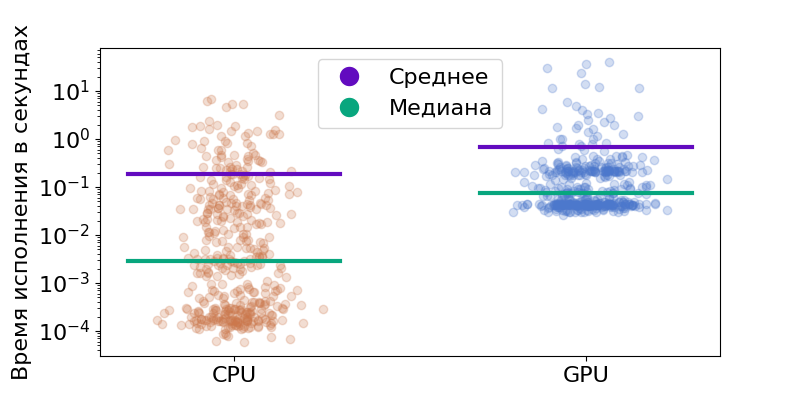
\includegraphics[scale = 0.85]{Cloud.png}
    \caption{Облако распределения времени исполнения запросов}
    \label{GraphicFull}
\end{figure}

\begin{figure}[H]
    \centering
    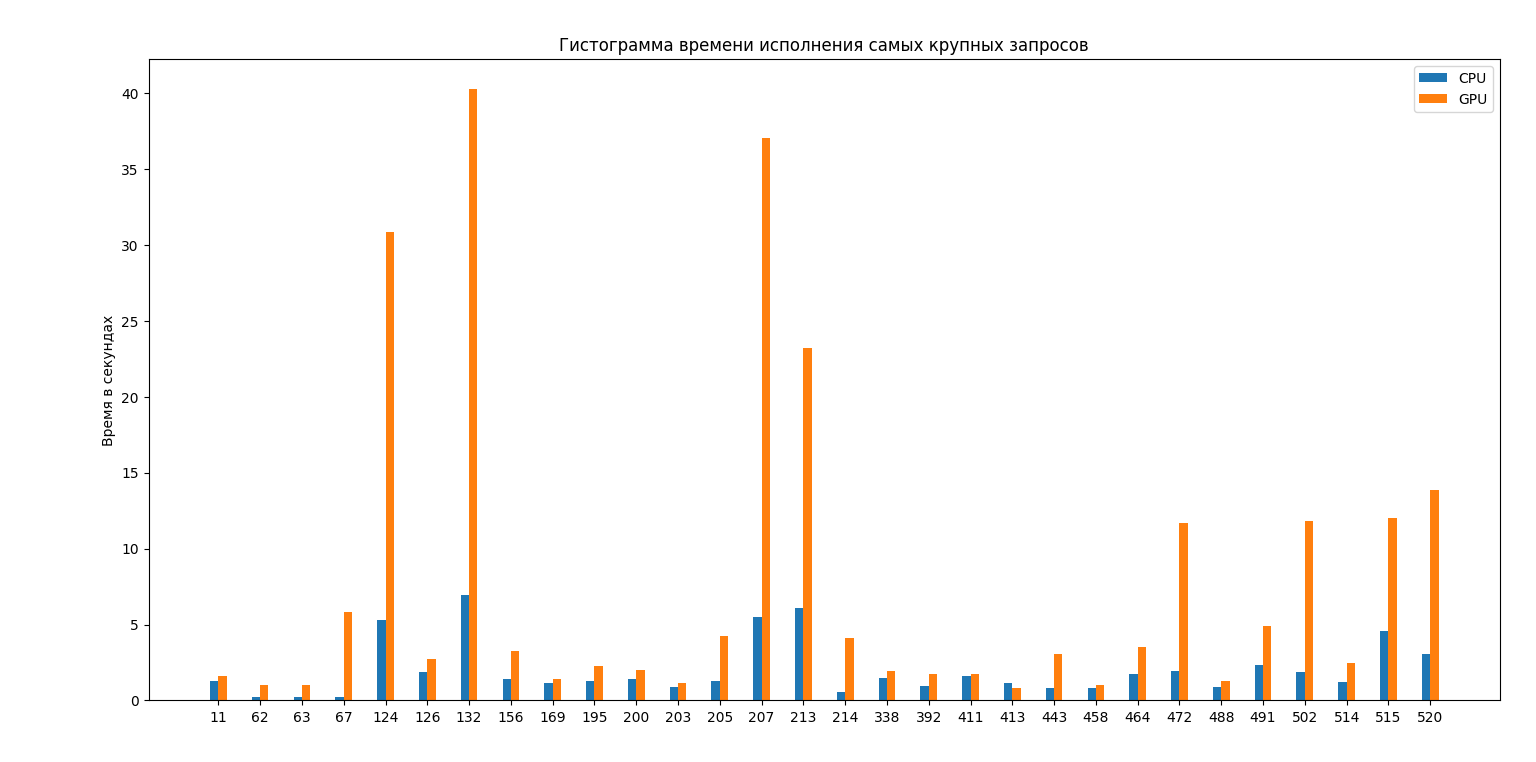
\includegraphics[scale = 0.42]{HistBig.png}
    \caption{Гистограмма времени исполнения самых крупных запросов (занявших более 1 секунды)}
    \label{GraphicBig}
\end{figure}

\newpage

Было построено облако распределения времени работы (Рис. \ref{GraphicFull}) реализаций на CPU и GPU на разных запросах. Заметно, что даже маленькие запросы реализация на GPU исполняет с некоторой задержкой. Так же была построена гистограмма для выборки самых крупных запросов, в которых время работы одной из реализации больше 1 секунды (Рис. \ref{GraphicBig}). Можно заметить, что есть отдельные запросы, на которых реализация на GPU работает намного хуже реализации на CPU. В дальнейшем следует подробнее изучить эти запросы и выявить закономерности.

Было посчитано среднее замедление, оно равняется 3.59. Этот показатель говорит о том, что текущая реализация алгоритма на GPU проигрывает реализации на CPU. Но есть и 20 запросов, на которых реализация на GPU выигрывает.

Для дальнейших исследований для каждого запроса было посчитано ускорение, взята медиана и посчитано среднее арифметическое: среднее арифметическое равняется 0.232, а медиана 0.0379. То, что медиана ускорений примерно в 8 раз меньше среднего показывает, что запросы делятся на те, на которых реализация на GPU проигрывает сильно, и те, на которых проигрыш не так заметен. Это также можно увидеть на графике (Рис. \ref{GraphicFull}).

Также были проанализированны лучшие и худшие показатели ускорения: взято среднее арифметическое по 5 лучшим (Таблица \ref{Best5Queries}) и 5 худшим (Таблица \ref{Worst5Queries}). У лучших этот показатель равняется 1.584, что говорит о том, что есть запросы, на которых реализация на GPU показывает себя значительно лучше реализации на CPU. Худший показатель же крайне мал: 0.000603. Это говорит о том, что есть отдельный тип запросов, с которыми реализация на GPU крайне плохо работает. Можно заметить, что время работы у алгоритма на CPU крайне мало, и возможно такая большая разница из-за того, что сама работа с GPU занимает всегда какое-то время, которое незначительно в более крупных запросах, но в таких малых превышает время вычислений.

\begin{table}[]
\centering
    \begin{tabular}{|c|c|c|c|}
    \hline
         Номер запроса & Время GPU & Время CPU & Ускорение \\
    \hline
        353 & 0.182 & 0.263 & 1.444 \\
        421 & 0.294 & 0.441 & 1.501 \\
        416 & 0.431 & 0.704 & 1.633 \\
        346 & 0.277 & 0.46  & 1.658 \\
        311 & 0.179 & 0.3   & 1.682 \\
    \hline
    \end{tabular}
    \caption{5 лучших запросов}
    \label{Best5Queries}
\end{table}

\begin{table}[]
\centering
    \begin{tabular}{|c|c|c|c|}
    \hline
         Номер запроса & Время GPU & Время CPU & Ускорение \\
    \hline
        429 & 0.170 & 0.000081 & 0.000476 \\
        511 & 0.200 & 0.000111 & 0.000553 \\
        484 & 0.202 & 0.000127 & 0.000627 \\
        433 & 0.175 & 0.000118 & 0.000671 \\
        442 & 0.174 & 0.000119 & 0.000683 \\
    \hline
    \end{tabular}
    \caption{5 худших запросов}
    \label{Worst5Queries}
\end{table}


Результаты эксперимента показали, что реализация алгоритма на GPU хорошо справляется с данными из реального мира, но при этом проигрывает в производительности реализации на CPU. Изучение среднего замедления показало, что среднее время исполнения запроса того же порядка, что и время исполнения запроса на CPU, а на некоторых запросах реализация на GPU показала себя даже лучше, следовательно реализацию на GPU можно использовать для распределения нагрузки на графические ускорители при многочисленных запросах. Анализ типов запросов, на которых реализация на GPU показывает себя лучше реализации на CPU или наоборот сильно ей проигрывает не был проведен, он планируется в дальнейших исследованиях алгоритма.  

